\section{Services Engagements: A Closer Look}

At the highest level, software services are of three kinds: consulting, systems integration, and application services. Consulting refers to business level consulting, in which domain experts work with a client to advise the client on major decisions and high-level design of a solution.  Systems integration refers to assembling a solution from off the shelf software and hardware components, with relatively little custom programming component.  We will focus only on application services---this is the kind that relates most closely to software engineering.  To make the setting concrete, we give an example of a service engagement that focuses on application services. 

Consider a large health-care management company that needs to make sure that their IT systems are compliant with a newly passed patient privacy legislation. Over the years, this company has accumulated a portfolio of a dozen applications implemented in a variety of technologies. It did not make business sense to keep in-house staff around to be able to make transformational changes to the application. The company decides to use a software services company to make this change. While they are at it, they decided to outsource support activities to the services company, to further reduce in house IT costs.  Vendors (i.e. services companies) are invited to submit proposals to transform the application suite, test it, and then continue to provide steady state maintenance service.

Software services vendors respond to the request for proposals with a plan of what they would do, along with the pricing. To differentiate themselves, they need to show the innovations that they bring to the table that help the health-care management company in terms of cost or quality. For example, a differentiator could be that the vendor has previously worked on similar transformational effort for another health-case management company, and were able to demonstrate 20\% reduction in IT support costs during steady state maintenance. Vendors also offer service-level agreements, so that the health-care management company can hedge their risk.  Typically service-level agreements would include financial charges if certain milestones are not met, or if support quality does not measure up to benchmarks. The vendors also need to do \textit{due diligence}, in which they assess their own risk in taking on the application portfolio from the health-care management company: the messier the portfolio, the more it would cost to transform and support it.

The winning vendor would then go through phases of transitioning, transformation, and steady-state maintenance; see Figure~\ref{fig:phases}. \textit{Transitioning} means taking over the application portfolio from its owner. Some amount of human-level knowledge transfer from the client to the vendor takes place by way of workshops, but typically, a lot of left for the vendor to discover from the available artifacts. In the \textit{transformation} phase, the client and the vendor collaborate to work out detailed requirements and the vendor allocates human resources to carry out the implementation and testing. The implementation and testing phases resemble a development or a legacy transformation project at a product company.  Finally, the transformed portfolio enters \textit{steady-state} maintenance phase, where field bugs are handled and customer support is provided.

The vendor relies heavily on \textit{knowledge management} through all these phases: the project must go on with as little as possible reliance on particular individuals who have an intimate knowledge of the application portfolio. Not only are the client's people unavailable, there is significant churn in the vendor's staff as well.

Additionally, a governance and risk management plan is put in effect for the entire lifecycle of the engagement, so both the client and the vendor are in sync and the continuation of the engagement makes business sense.

Services engagements vary widely: a company could use multiple vendors to carry out the work: e.g. one vendor for implementation, another for testing, and yet another for steady-state maintenance.  And while this example was in the context of an existing application portfolio, sometimes services engagement start from design and build phase, a.k.a. a ``green field" project.

%Consulting vs. Systems integration vs. Application Services.

%Design and build.
%
%Enhancements.
%
%Maintenance.
%
%Talk about organization of vendors. By service lines? By industry? By technologies? Look at Steve Kagan's white paper.

\begin{figure}[t]
\centering
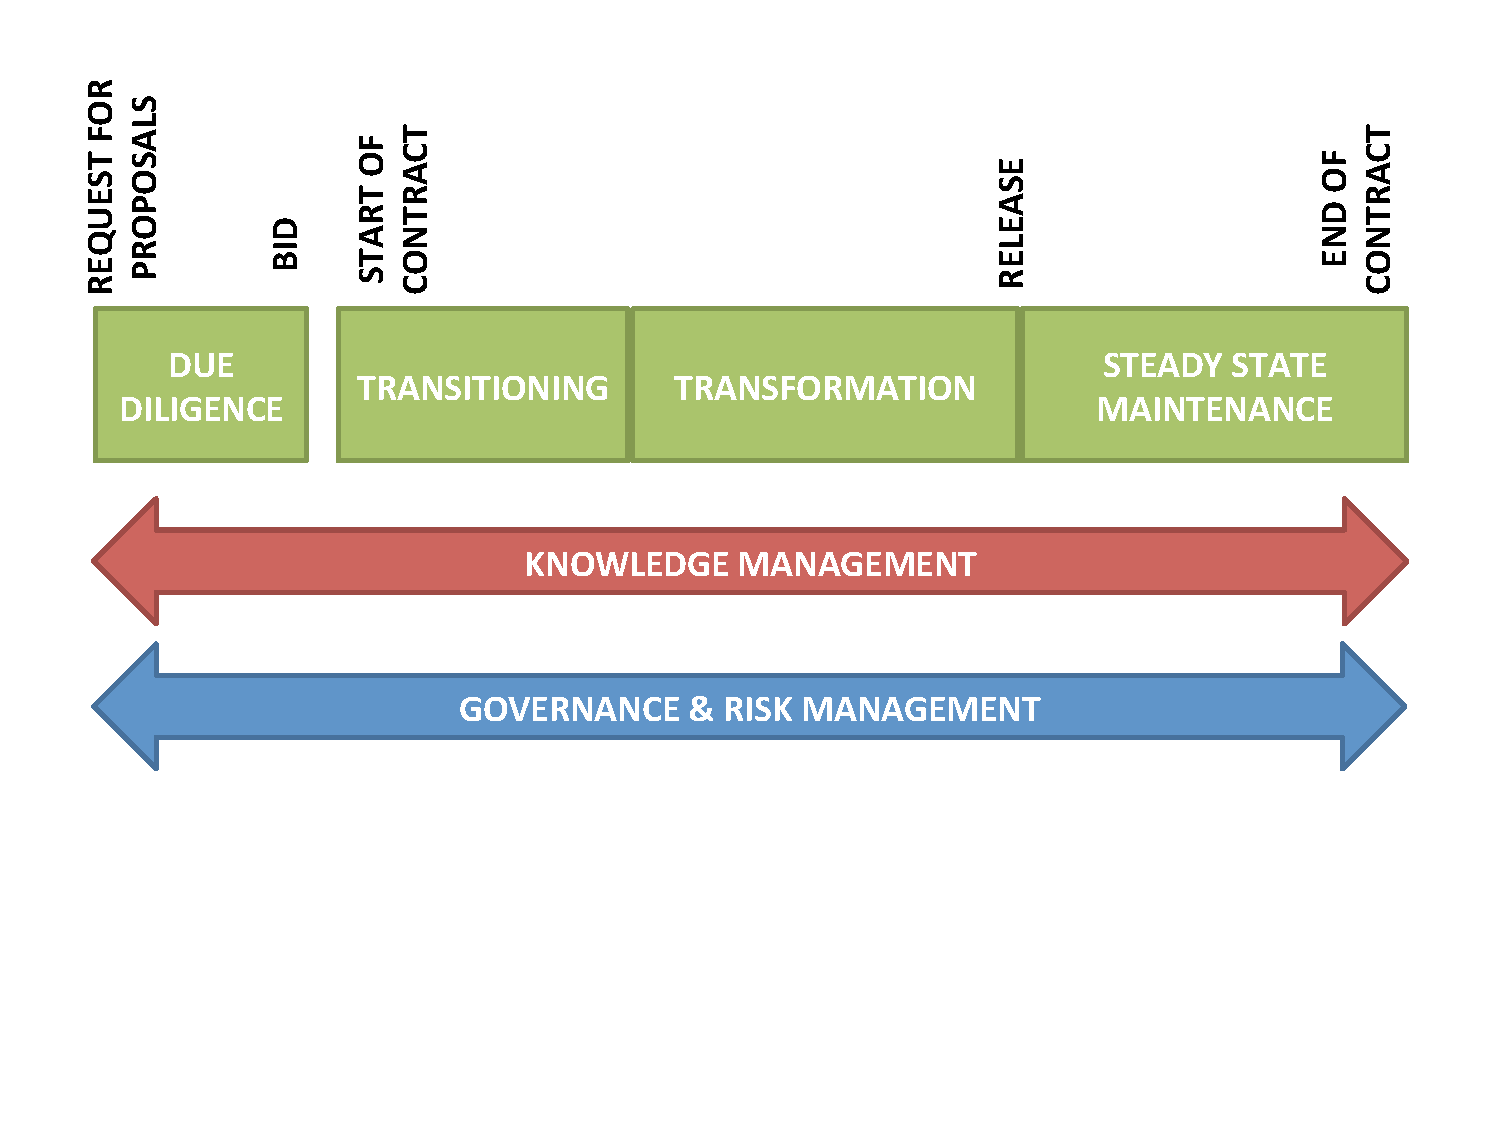
\includegraphics[width=0.9\columnwidth, clip, trim = 0mm 50mm 0mm
  17mm]{figs/phases.pdf}
\vspace*{-15pt}
\caption{Typical software services engagement.}
\vspace*{-10pt}
\label{fig:phases}
\end{figure}


